\documentclass{article}
\usepackage[utf8]{inputenc}
\usepackage{graphicx}
\usepackage{amsmath}

\title{Neural Network}
\author{Steven Wang}
\date{March 2021}

\begin{document}

\maketitle

\[
\hspace*{-15mm}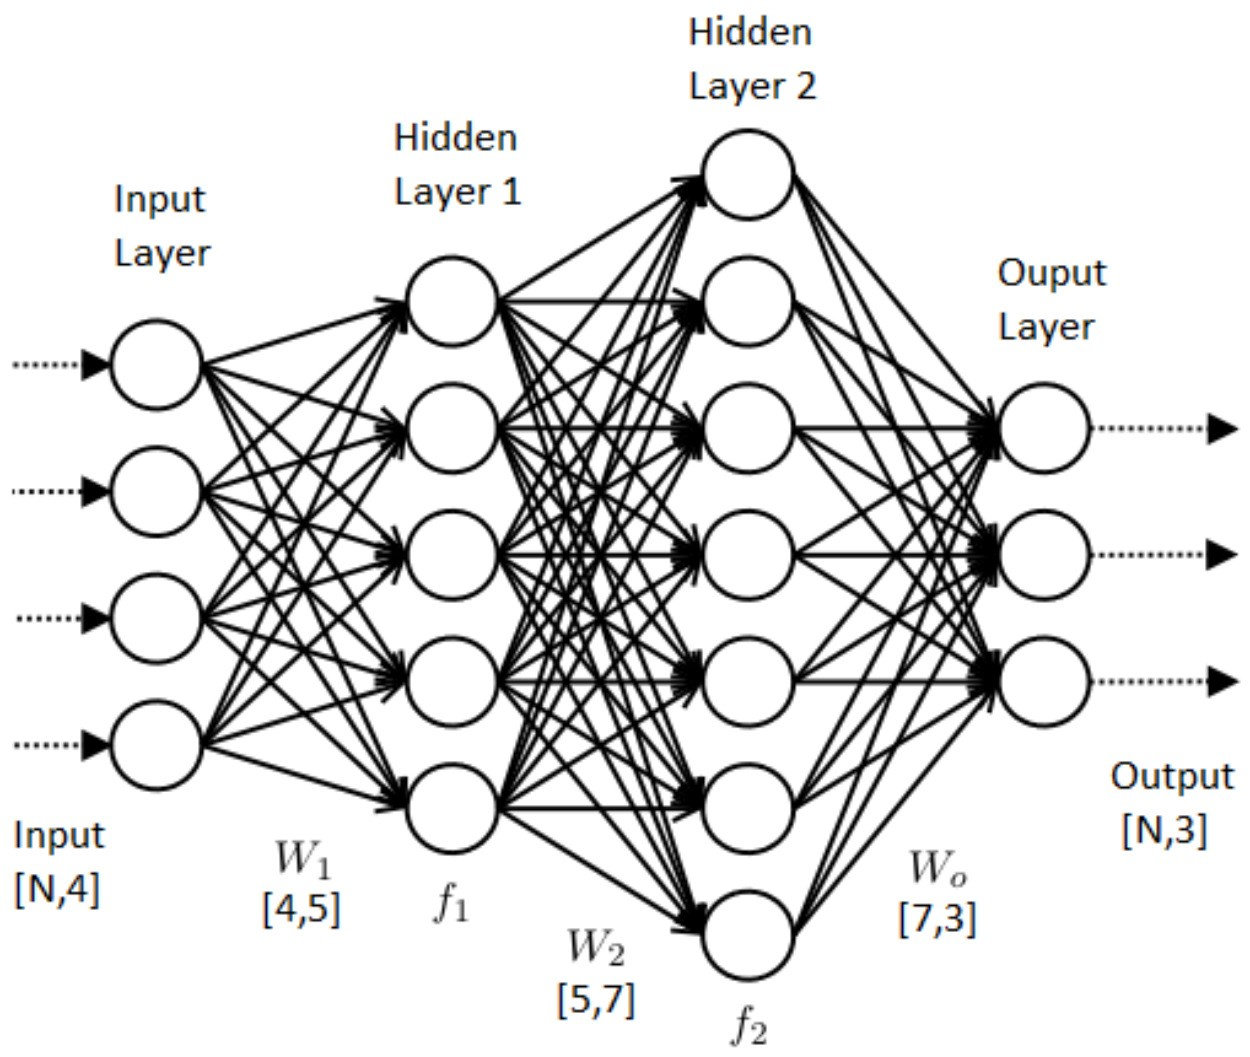
\includegraphics[scale=0.35]{neural_netowrk}
\]

\section{Definition of "Neuron"}

\begin{enumerate}
    \item A function which takes input of previous layers $activation\ value^{[2,\ see\ the\ following\ line]}$ and output its own activation value.
    \item The value of each neuron's output is called \textbf{activation}(usually between 0 and 1).
    \item For one specific neuron: the function usually takes form like:
  
        $$layer\ 1\ activation * weights + bias$$

        which can also be expressed as $$w_1*a_1 + w_2*a_2 + ... + w_n*a_n + bias$$
    
        \begin{enumerate}
            \item \textbf{weight}: level of impact of the previous layer activation has on the current layer neuron. You think think this as the link between neurons.
            \item \textbf{bias}: An added value to the weighted sum of previous layer activation. You can think this as a threshold of when to activate the neuron. e.g. If the bias is a relaively large negative value, you don't want this neuron to be activated easily.
        
        \end{enumerate}

    \item It is often desirable to make the activation between 0 and 1. To do so we often use a function to tweak the output value to align with our expectation. Like a sigmoid function $\sigma()$ (logistic curve).
  
    \item In practice, sigmoid function is difficult to train. Pracitioners often use rectifier function(f(x) = max(0,x)). A unit employing the rectifier is also called a rectified linear unit (\textbf{ReLU}).
  
\end{enumerate}

    \textbf{Machine learning is the practice of finding the right weights and biases.}

        $$a^{(L)} = \sigma(w^{(L)}a^{(L-1)}+b^{(L)})$$ \\
        \indent $a$: activation \\
        \indent $w$: weight \\
        \indent $b$: bias \\
        \indent $\sigma()$: sigmoid function \\
        \indent The upper right notation of $a^{\textbf{(L)}}$ is to differentiate layers.
 

\section{Gradient Descent}
    \begin{enumerate}
        \item To start, we initialize all the weights and biases randomly.
        \item Define the cost funciton which computes the cost. The higher the cost, the less desirable the output. We want the Nerual Network model to have the lowest cost given a cost function, which means high model accuracy. The cost function should output a single number.
            $$f(weights, biases | input)=\hat{activation}$$
            cost is:
            $$\Sigma_{i=0}^n(\hat{activation}_i - y_i)^2$$
            here $y$ is the desired output provided beforehand. We denote cost function as:
            $$ C(w,b) = (f(w,b)-y)^2 $$

    \textbf{Machine learning is minimizing the cost function.}
    
        \item To achieve the minimization of the cost function, we use a technique called \textbf{gradient descent}, which can be thought as calculating negative dirivative of weights and biases and get local minimum.
    \end{enumerate}

\section{Back Propagation}
    Definition: Algorithm of how a single training example would like to change the weights and biases, namely how to get better negative gradient descent. To simply the idea: 
        \begin{enumerate}
            \item For a single training example, the Neural Network model will output a result, either a good one or a bad one. We want to improve the result (lower the cost).
            \item For any given layer, there are three things(inputs) we can change to alter the output:
                \begin{enumerate}
                    \item $a^{(i-1)}$: previous layer activation
                    \item $w^{(i)}$: weights
                    \item $b^{(i)}$: biases
                \end{enumerate}
            \item We want to change the weights($w^{(i)}$) and biases($b^{(i)}$) for the currect layer accordingly.
            \item We also want to change previous layer activation ($a^{(i-1)}$) accordingly. To do so we just repeat step 1, 2 and 3, hence the name \textbf{back propagation}.
        \end{enumerate}

\section{Math \& Notation of Back Propagation}
    \textbf{* Assume for now that there is only one neuron in each layer of the Neural Network}
    \begin{enumerate}
        \item $a^{(L)}$: activation of layer $L$
        \item $w^{(L)}$: weights of layer $L$
        \item $b^{(L)}$: biases of layer $L$
        \item $$z^{(L)}=w^{(L)}a^{(L-1)}+b^{(L)}$$
 $$a^{(L)}=\sigma(w^{(L)}a^{(L-1)}+b^{(L)})=\sigma(z^{(L)})$$
        \item $y$: desired output
        \item Cost function of a specific training example: $$C_0=(a^{(L)}-y)^2$$
        \item $$\frac{\partial C_0}{\partial w^{(L)}}=\frac{\partial z^{(L)}}{\partial w^{(L)}} \frac{\partial a^{(L)}}{\partial z^{(L)}} \frac{\partial C_0}{\partial a^{(L)}}$$
        \item $$\frac{\partial C_0}{\partial a^{(L)}}=2(a^{(L)}-y)$$
        \item $$\frac{\partial a^{(L)}}{\partial z^{(L)}}=\sigma'(z^{(L)})$$
        \item $$\frac{\partial z^{(L)}}{\partial w^{(L)}}=a^{(L-1)}$$
        \item $$\frac{\partial C_0}{\partial w^{(L)}}=a^{(L-1)}\sigma'(z^{(L)})2(a^{(L)}-y)$$
        \item $$\frac{\partial C_0}{\partial b^{(L)}}=\frac{\partial z^{(L)}}{\partial b^{(L)}} \frac{\partial a^{(L)}}{\partial z^{(L)}} \frac{\partial C_0}{\partial a^{(L)}}$$
        \item $$\frac{\partial C_0}{\partial b^{(L)}}=1\cdot\sigma'(z^{(L)})2(a^{(L)}-y)$$
        \item $$\frac{\partial C_0}{\partial a^{(L-1)}}=w^{(L)}\sigma'(z^{(L)})2(a^{(L)}-y)$$
        \item Cost of all training examples is the average of all: $$\frac{\partial C}{\partial w^{(L)}}=\frac{1}{n}\sum^{n-1}_{k=0}\frac{\partial C_k}{\partial w^{(L)}}$$
        \item $$\nabla C = 
            \begin{bmatrix}
                \frac{\partial C}{\partial w^{(1)}} \\
                \frac{\partial C}{\partial b^{(1)}} \\
                \vdots \\
                \frac{\partial C}{\partial w^{(L)}} \\
                \frac{\partial C}{\partial b^{(L)}} \\
            \end{bmatrix}$$
    \end{enumerate}

    \textbf{* Now assume there are multiple neurons for each layer}
    \begin{enumerate}
        \item $k$: $k$th neuron of layer $(L-1)$
        \item $j$: $j$th neuron of layer $(L)$
        \item $a^{(L)}_{j}$: $j$th activation of layer $(L)$
        \item $w^{(L)}_{jk}$: weight of $k$th activation of layer $(L-1)$ on $j$th activation of layer $(L)$
        \item $b^{(L)}_{jk}$: bias of $w^{(L)}_{jk}$
        \item Cost function of a specific training example: $$C_0=\sum^{n_L-1}_{j=0}(a^{(L)}_{j}-y_j)^2$$
        \item $$z^{(L)}_{j}=...+w^{(L)}_{jk}a^{(L-1)}_{j}+...+b^{(L)}_{j}$$
        \item $$a^{(L)}_{j}=\sigma(z^{(L)}_{j})$$
        \item $$\frac{\partial C_0}{\partial w^{(L)}_{jk}}=\frac{\partial z^{(L)}_{j}}{\partial w^{(L)}_{jk}} \frac{\partial a^{(L)}_{j}}{\partial z^{(L)}_{j}} \frac{\partial C_0}{\partial a^{(L)}_{j}}$$
        \item $$\frac{\partial C_0}{\partial a^{(L-1)}_{k}}=\sum^{n_{L-1}}_{j=0}\frac{\partial z^{(L)}_{j}}{\partial a^{(L-1)}_{k}} \frac{\partial a^{(L)}_{j}}{\partial z^{(L)}_{j}} \frac{\partial C_0}{\partial a^{(L)}_{j}}$$


    \end{enumerate}

\section{Final formula of Back Propagation}
    \begin{enumerate}
        \item $$\nabla C=\frac{\partial C}{\partial w^{(l)}_{jk}}=a^{(l-1)}_{k}\sigma'(z^{(l)}_{j})\boxed{\frac{\partial C}{\partial a^{(l)}_{j}}}$$
        \item $$\boxed{\frac{\partial C}{\partial a^{(l)}_{j}}}=\sum^{n_{l+1}-1}_{j=0}\frac{\partial z^{(l+1)}_{j}}{\partial a^{(l+1)}_{k}} \frac{\partial a^{(l+1)}_{j}}{\partial z^{(l+1)}_{j}} \frac{\partial C}{\partial a^{(l+1)}_{j}}=w^{l+1}_{jk} \sigma'(z^{l+1}_{j}) \frac{\partial C}{\partial a^{(l+1)}_{j}}$$
    \end{enumerate}
    
\end{document}

